\documentclass[english]{article}
\usepackage[T1]{fontenc}
\usepackage[latin9]{inputenc}
\usepackage{geometry}
\geometry{verbose,tmargin=2.54cm,bmargin=2.54cm,lmargin=2.17cm,rmargin=2.17cm}
\usepackage{amstext}
\usepackage{stackrel}
\usepackage{graphicx}
\usepackage{setspace}
\onehalfspacing
\usepackage{babel}
\begin{document}

\title{Prediction of Stock Market with Sentiment Analysis}

\author{Lin Zeng(lz447), Qin Lu(ql224), Sizhang Zhao(sz459)}

\date{October 27, 2016}
\maketitle

\section{Idea}
\begin{quotation}
Stock market prediction is the core research area in trading and investment.
Stock price is determined by the behavior of human investors, and
the investers determine stock prices by using publicly available information
to predict the market future trend. Financial news can thus play a
significant role in influencing the stock trend as human react to
the information. Previous reasearch have suggested that there is some
lag between the time news article was released and the time the market
absorbed and reflected these information. So our main goal here is
to classify the news as our sentiment factor and use the sentiment
factor to determine the impact of the news on the stock price. 

In our research, we focus on sentiment analysis with Google news in
stocks division, and build up machine learning models to measure the
relationship between news sentiment and stock index trend(DJIA) over
time. Finally, we try to design a tradable portfolio based on our
sentiment factor and test its application in investments. 
\end{quotation}

\section{Data Scraping}
\begin{quotation}
Headers of financial news usually contain the impact of a certain
event to the whole market. For example, \emph{warn, volatility, decline,
plunge} are common phrases that are conceived as negative news to
market, and \emph{hike, allow, optimism, gain} are phrases that are
considered as positive ones. So in order to capture as much sentiment
information as possible for news each day, we use the headers of financial
news as our data set instead of the whole article.

We designe a web scraper to scratch the Google news headers in stock
division from January 2007 - December 2009 and January 2013- December
2015 in daily basis. 

By locating the headers in source code from Google news, we use \emph{BeautifulSoup}
package in Python to scratch the headers in the search page by changing
the time zone in advanced search. We store news headers scratched
from Google news each day in separate \emph{.txt} file as the raw
data for sentiment analysis. 

In addition, we alter the news search criterion by industry to predict
the specific industry trend. For example, we search\emph{ real estate}
instead of\emph{ stock} to obtain specific industry news in predicting
real estate index future trend.

We also download the \emph{Dow Jones Industrial Average} (DJIA) as
our response variable data from Yahoo Finance.
\begin{center}
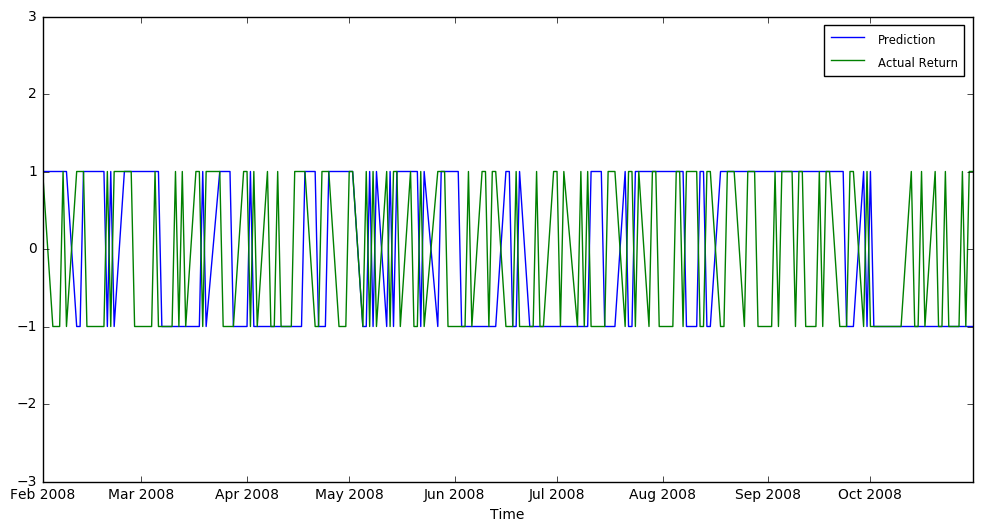
\includegraphics[scale=0.25]{1}
\par\end{center}
\begin{center}
Figure 1: Source code and the search page of Google news
\par\end{center}
\begin{center}
{\large{}$\Downarrow$}
\par\end{center}{\large \par}
\begin{center}
\includegraphics[scale=0.4]{2}
\par\end{center}
\begin{center}
Figure 2: News headers stored in .txt file by our web scraper
\par\end{center}
\end{quotation}

\section{Sentiment Analysis with Stock News}
\begin{quotation}
Our goal here is to develop a system capable of providing information
about the polarity in our scratched news documents. \emph{OpinionFinder}(OF)
is a publicly available software package that processes documents
and automatically identifies subjective sentences and sentiment expresssions.
The subjectivity analysis provides us three polarity level: \emph{positive},
\emph{neutral}, \emph{negative}. 

The polarity classifier takes clues consisting of words with a prior
polarity of \emph{positive}, \emph{negative} or \emph{neutral} (for
example,\emph{ hike}, \emph{drop}, \emph{indicate}, repectively) and
thus uses a modified version of the classifier described in Wilson
et al. (2005) to determine the contextual polarity of the clues. Heuristics
were used to improve the speed of the classifier so it no longer needs
the dependency parse output. When evaluated on the MPQA opinion corpus,
the overall accuracy is 73.4\%.

After obtaining the polarity word list, we mark positive words as
1, neutral as 0 and negative as -1, and take the average of them as
our sentiment factor. The sample output of OF is demonstrated as follow.
\begin{center}
\includegraphics[scale=0.5]{3}
\par\end{center}
\begin{center}
Figure 3: Sample output of OpinionFinder
\par\end{center}
\end{quotation}

\section{Granger Causality Analysis}
\begin{quotation}
We are concerned with the question whether the changes in our sentiment
factor is correlated with changes in the stock market, in particular
DJIA closing values. To answer this question, we apply the econometric
technique of Granger causality analysis to the daily time series produced
by sentiment factor and the DJIA. Granger causality analysis rests
on the assumption that if a variable $X$ causes $Y$ then changes
in $X$ will systematically occur before changes in $Y$. We will
thus find that the lagged values of $X$ will exhibit a statistically
significant correlation with $Y$. We are not testing actual causation
but whether one time series has predictive information about the other
or not. 

Our DJIA time series, denoted as $D_{t}$, is the adjusted close price
of DIJA at time $t$. To test whether our sentiment factor time series
predicts the changes in stock market value, we compare the variance
explained by two linear models as show below. The first model ($L_{1}$)
uses only the lagged value $D_{t-1}$, while the second model ($L_{2}$)
uses the lagged value $D_{t-1}$ and the 3 lagged values of sentiment
factor $X_{t-1},X_{t-2},X_{t-3}$.
\begin{center}
$L_{1}:\,D_{t}=\alpha+\stackrel[i=1]{3}{\sum}\beta_{i}D_{t-i}+\varepsilon_{t}$
\par\end{center}
\begin{center}
$L_{2}:\,D_{t}=\alpha+\stackrel[i=1]{3}{\sum}\beta_{i}D_{t-i}+\stackrel[i=1]{3}{\sum}\gamma_{i}D_{t-i}+\varepsilon_{t\text{}}$
\par\end{center}
The results are shown below indicating the adjusted $R^{2}$ of $L_{2}$
is larger than $L_{1}$, this means Granger causality analysis suggests
a predictive relation between certain sentiment dimensions and DJIA.
\begin{center}
\includegraphics[scale=0.4]{5}\includegraphics[scale=0.4]{4}
\par\end{center}
\begin{center}
Figure 4: $L_{1}$ regression summary$\qquad\qquad$ Figure 5: $L_{2}$
regression summary
\par\end{center}
\begin{center}
\includegraphics[scale=0.4]{6}
\par\end{center}
\begin{center}
Figure 6: $L_{1},L_{2}$ prediction of DJIA and true DJIA (normalized)
\par\end{center}
\end{quotation}

\section{Next Step}
\begin{quotation}
Our Granger causality analysis suggests a predictive relation between
certain sentiment dimensions and DJIA. However, Granger causality
analysis is based on linear regression whereas the relation between
the market sentiment and stock market value is almost certainly non-linear.
To better addree these non-linear effects and assess the contribution
that sentiment factor can make in predictive models of DJIA values,
we will compare the performance of a \emph{Self-organizing Fuzzy Neural
Network} (SOFNN) model that predicts DJIA values on the basis of two
sets of inputs: 
\begin{itemize}
\item The past 3 days of DJIA values 
\item the same combined with the sentiment factors
\end{itemize}
Statistically significant performance differences will allow us to
either confirm or reject the null hypothesis that market sentiment
measurement do not improve predictive models of DJIA values.

We use a SOFNN as our prediction model since they have previously
been used to decode nonlinear time series data which describe the
characteristics of the stock market and predict its values. Our SOFNN
in particular is a five- layer hybrid neural network with the ability
to self-organize its own neurons in the learning process. 

Having predicted the DJIA closing values one day in advance, we can
use these predicted values to make sell/buy decisions. We develop
a naive greedy strategy based on a simple assumption that we can hold
at most one stock at any given time. Following are steps of our strategy(to
be tested):
\begin{itemize}
\item Pre-computation

We maintain a running average and standard deviation of actual adjusted
stock values of previous $k$ days
\item Sell Decision

If the predicted stock value for the next day is $n$ standard deviation
less than the mean, we sell the stock else we hold.
\item Buy Decision

If the predicted stock value is $m$ standard deviation more than
the actual adjusted value at buy time, we buy the stock else we hold.
\end{itemize}
\end{quotation}

\end{document}
